% DOCUMENT CLASS SETUP
\documentclass[12pt, a4paper]{article}

% DOCUMENT PACKAGES
\usepackage[a4paper, margin=1in]{geometry}
\usepackage{titling}
\usepackage{enumitem}
\usepackage{amsmath}
\usepackage{amssymb}
\usepackage{mathtools}
\usepackage{graphicx}
\usepackage{xcolor}
\usepackage{listings}
\usepackage{hyperref}
\usepackage{csquotes}

% FONT AND ENCODING SETUP
\usepackage{fontspec}
\usepackage{polyglossia}
\usepackage[Thai]{ucharclasses}
\setdefaultlanguage{english}
\setotherlanguage{thai}
\setTransitionsFor{Thai}{\thaifont}{\normalfont}
\newfontfamily{\thaifont}{THSarabun.ttf}[
    Path=./,
    BoldFont=THSarabunBold.ttf,
    ItalicFont=THSarabunItalic.ttf,
    BoldItalicFont=THSarabunBoldItalic.ttf,
    Scale=1.23
]
\XeTeXlinebreaklocale "th"
\XeTeXlinebreakskip = 0pt plus 1pt

% PROFESSIONAL CODE BLOCK
\usepackage{tcolorbox}
\tcbuselibrary{minted, skins, breakable}

% DEFINE GITHUB DARK THEME COLORS %
\definecolor{ghback}{HTML}{0d1117}    % Dark background
\definecolor{ghtext}{HTML}{c9d1d9}    % Light gray text
\definecolor{ghborder}{HTML}{30363d}  % GitHub Border color

% PROFESSIONAL CODE BLOCK CONFIGURATION (MINTED VERSION) %
\renewcommand{\theFancyVerbLine}{\textcolor{white!60!gray}{\scriptsize\arabic{FancyVerbLine}}}
\newtcblisting{codeblock}[2][]{
    enhanced,
    breakable,
    colback=ghback,
    colframe=ghborder,
    coltitle=ghtext,
    colupper=ghtext,
    fonttitle=\bfseries\small,
    arc=3mm,
    boxrule=0.5mm,
    % PADDING SETTINGS
    left=25pt,
    right=10pt,
    top=5pt,
    bottom=5pt,
    % MINTED SETTINGS
    listing engine=minted,
    listing only,
    minted language=python,
    minted options={
        linenos,
        numbersep=5pt,
        fontsize=\footnotesize,
        breaklines=true,
        breakanywhere=true,
        autogobble,
        style=monokai,
    },
    title={#2},
    #1
}

% DOCUMENT TITLE SETUP %
\title {
	\textbf{2110573 PATTERN RECOGNITION} \\
    \vspace{1em}
	\Large{\textbf{Take-Home Midterm Exam}} \\
    \vspace{0.5em}
    \large{Computer Engineering, Chulalongkorn Univerity}
}
\author{Worralop Srichainont}
\date{\today}
\setlength{\droptitle}{15em}

% DOCUMENT CONTENTS
\begin{document}

    \maketitle
    \thispagestyle{empty}
    \clearpage

    \tableofcontents
    \thispagestyle{empty}
    \clearpage

    \pagenumbering{arabic}

    \section{Problem 1 (20 Points)}
        You recorded the performance of a computer vision model for screening faulty parts in a certain factory. The results are as shown in the table below.
        \begin{table}[h]
            \centering
            \begin{tabular}{|c|c|c|}
                \hline
                \textbf{Actual / Model} & \textbf{Good parts (Model)} & \textbf{Good parts (Model)} \\
                \hline \hline
                \textbf{Good parts (Actual)} & 350 & 150 \\
                \hline
                \textbf{Bad parts (Actual)} & 5 & 45 \\
                \hline
            \end{tabular}
        \end{table}

        \subsection{Problem 1.1. (4 Points)}
            What should be the positive class (Good parts or Bad parts)? Why?

            \vspace{1em}

            \noindent \underline{\textbf{Ans.}} \textbf{The bad parts} should be the positive class because the objective of the computer vision model is to identify the faulty parts (or bad parts) in a factory.

        \subsection{Problem 1.2. (6 Points)}
            Calculate the accuracy, precision, recall, F1 score, true positive rate, and false alarm rate of the model.

            \vspace{1em}

            \noindent \underline{\textbf{Solution}}
            
            \noindent First of all, consider these following values
            \begin{itemize}
                \item \textbf{True Positive (TP)} means predicted bad parts, actual bad parts. (45 predictions)
                \item \textbf{False Positive (FP)} means predicted bad parts, actual good parts. \\ (150 predictions)
                \item \textbf{True Negative (TN)} means predicted good parts, actual good parts. \\ (350 predictions)
                \item \textbf{False Negative (FN)} means predicted good parts, actual bad parts. \\ (5 predictions)
            \end{itemize}
            \begin{align*}
                \intertext{Calculate the accuracy of the model}
                \text{Accuracy} &= \frac{\text{TP} + \text{TN}}{\text{TP} + \text{FP} + \text{TN} + \text{FN}} \\[1em]
                \text{Accuracy} &= \frac{45 + 350}{45 + 150 + 350 + 5} \approx 0.718 \\[1em]
                \intertext{Calculate the precision of the model}
                \text{Precision} &= \frac{\text{TP}}{\text{TP} + \text{FP}} \\[1em]
                \text{Precision} &= \frac{45}{45 + 150} \approx 0.231 \\[1em]
                \intertext{Calculate the recall (true positive rate) of the model}
                \text{Recall} &= \frac{\text{TP}}{\text{TP} + \text{FN}} \\[1em]
                \text{Recall} &= \frac{45}{45 + 5} = 0.900 \\[1em]
                \intertext{Calculate the F1 score of the model}
                \text{F1 Score} &= 2 \times \frac{\text{Precision} \times \text{Recall}}{\text{Precision} + \text{Recall}} \\[1em]
                \text{F1 Score} &= 2 \times \frac{\frac{3}{13} \times \frac{9}{10}}{\frac{3}{13} + \frac{9}{10}} \approx 0.367 \\[1em]
                \intertext{Calculate the false alarm rate of the model}
                \text{Recall} &= \frac{\text{FP}}{\text{FP} + \text{TN}} \\[1em]
                \text{Recall} &= \frac{150}{150 + 350} = 0.300
            \end{align*}

            \noindent \underline{\textbf{Answer}}
            \begin{table}[h]
                \centering
                \begin{tabular}{|c|c|}
                    \hline
                    \textbf{Metrics} & \textbf{Value} \\
                    \hline \hline
                    Accuracy & 0.718 \\
                    Precision & 0.231 \\
                    Recall & 0.900 \\
                    F1 Score & 0.367 \\
                    True Positive Rate & 0.900 \\
                    False Alarm Rate & 0.300 \\
                    \hline
                \end{tabular}
            \end{table}

        \subsection{Problem 1.3. (5 Points)}
            If IBM offers to sell the factory a better computer vision model. They claim that their model obtains 90\% recall and 30\% precision.
            Should you switch to use IBM's model? Why or why not?
            What other information might be helpful in determining this answer?

            \vspace{1em}

            \noindent \underline{\textbf{Ans.}} The objective of the model is to detect faulty parts so the recall must as high as possible,
            because the false negative has much more negative impact than the false positive on factory revenue.

            Since the original model and the IBM's model has equal recall, but the IBM's model has higher precision which causes the F1 score
            to improve from 0.367 to 0.450. \textbf{Therefore, the answer is I would switch to the IBM's model}.

    \pagebreak

        \subsection{Problem 1.4. (5 Points)}
            The cost of misclassifying a good part as a bad part is 10 dollars (discarding good material).
            The reputation cost of selling a defective part is 100 dollars.
            The current model takes in an image, $\mathbf{x}$, and output a score, $\mathbf{s}$, that is compared against a threshold, $\mathbf{t}$.

            If $\mathbf{s > t}$, it is declared as failed. Otherwise, it is considered as passed.
            The current settings of the factory sets $\mathbf{t}$ to 3. From the provide information, is $\mathbf{t}$ set properly? Why?
            If not, how should we change $\mathbf{t}$ relative to its original value?

            \vspace{1em}

            \noindent \underline{\textbf{Answer}}

            \vspace{0.5em}

            \textbf{The $t$ value is not set properly},
            because of the score $\mathbf{s}$ is not normalized in the finite range $[0, 1]$ which is hard to interpret and minimize damage cost.

            To set the threshold $\mathbf{t}$, we take the sigmoid function $\sigma(x)$ to convert raw score to class probability which in the range $[0, 1]$.

            $$\sigma(x) = \frac{1}{1 - e^{-x}}$$

            After converting into class probability, we consider the expected damage cost when perform a prediction to properly set the threshold $\mathbf{t}$.

            To calculate expected damage cost of predict the given part as bad parts (positive), we need to consider these two cases.
            \begin{itemize}
                \item \textbf{True Positive (TP)} has no damage cost.
                \item \textbf{False Positive (FP)} calculated by multiply the probability of the given part is good part by the damage cost which is \$10.
            \end{itemize}
            \begin{align*}
                E[\text{Damage Cost} | \text{Predict} = \text{Bad}] &= P(\text{Good} | x) \times {\text{Damage Cost}}_{\text{FP}} \\
                E[\text{Damage Cost} | \text{Predict} = \text{Bad}] &= P(\text{Good} | x) \times 10 \\
            \end{align*}

            To calculate expected damage cost of predict the given part as good parts (negative), we need to consider these two cases.
            \begin{itemize}
                \item \textbf{True Negative (TN)} has no damage cost.
                \item \textbf{False Negative (FN)} calculated by multiply the probability of the given part is good part by the damage cost which is \$100.
            \end{itemize}
            \begin{align*}
                E[\text{Damage Cost} | \text{Predict} = \text{Good}] &= P(\text{Bad} | x) \times {\text{Damage Cost}}_{\text{FN}} \\
                E[\text{Damage Cost} | \text{Predict} = \text{Good}] &= P(\text{Bad} | x) \times 100 \\
            \end{align*}

    \pagebreak

            Then calculate the probability of the given part is a bad parts at the point where the expected damage cost of the positive and negative prediction are equal.
            \begin{align*}
                E[\text{Damage Cost} | \text{Predict} = \text{Bad}] &= E[\text{Damage Cost} | \text{Predict} = \text{Good}] \\
                P(\text{Good} | x) \times 10 &= P(\text{Bad} | x) \times 100 \\
                P(\text{Good} | x) &= 10 \cdot P(\text{Bad} | x) \\
                1 - P(\text{Bad} | x) &= 10 \cdot P(\text{Bad} | x) \\
                11 \cdot P(\text{Bad} | x) &= 1 \\
                P(\text{Bad} | x) &= \frac{1}{11}
            \end{align*}

            From the equation above, we can conclude that the threshold probability where the damage cost of
            false positive and false negative are balanced is $P(\text{Bad} | x) = \frac{1}{11}$.
            \textbf{Therefore, the threshold} $\mathbf{t}$ \textbf{should be set at} $\mathbf{\frac{1}{11}}$
            \begin{align*}
                \text{Predicted Class} =
                \begin{dcases}
                    \text{Good parts (Negative)} & \text{if } \sigma(s) \leq \frac{1}{11} \\
                    \text{Bad parts (Positive)} & \text{if } \sigma(s) > \frac{1}{11}
                \end{dcases}
            \end{align*}

    \pagebreak

    \section{Problem 2 (15 Points)}
        You are starting a company to classify apples into good and bad ones. Given some data based on human experts.
        You try to build a machine learning model (Naive Bayes) from this data.

        \begin{table}[h]
            \centering
            \begin{tabular}{|c|c|c|c|}
                \hline
                \textbf{Class} & \textbf{Color} & \textbf{Weight} & \textbf{Sweetness} \\
                \hline \hline
                Good & Green & H & T \\
                Bad  & Red   & M & F \\
                Good & Red   & M & T \\
                Bad  & Green & L & T \\
                Good & Red   & M & T \\
                Good & Green & M & F \\
                Bad  & Red   & L & F \\
                Bad  & Red   & L & T \\
                Good & Red   & L & F \\
                Bad  & Red   & H & F \\
                \hline
            \end{tabular}
        \end{table}

        \subsection{Problem 2.1. (2 Points)}
            From the data, what is the prior probability for the two classes $P(\text{Good})$ and $P(\text{Bad})$?

            \vspace{1em}

            \noindent \underline{\textbf{Ans.}} $P(\text{Good}) = \frac{5}{10}$ and $P(\text{Bad}) = \frac{5}{10}$

        \subsection{Problem 2.2. (2 Points)}
            What is $P(\text{Good} | \text{Green})$ and $P(\text{Bad}| \text{Green})$?

            \vspace{1em}

            \noindent \underline{\textbf{Ans.}} To calculate those probabilities, consider only rows with \enquote{Green} value on the \enquote{Color} column.
            The result are $\mathbf{P(\textbf{Good} | \textbf{Green}) = \frac{2}{3}}$ and $\mathbf{P(\textbf{Bad} | \textbf{Green}) = \frac{1}{3}}$

        \subsection{Problem 2.3. (2 Points)}
            What is $P(\text{Green} | \text{Good})$ and $P(\text{Green}| \text{Bad})$?

            \vspace{1em}

            \noindent \underline{\textbf{Ans.}} Considering only rows with \enquote{Good} value on the \enquote{Class} column, we can calculate the
            probability $\mathbf{P(\textbf{Green} | \textbf{Good}) = \frac{2}{5}}$ \\[0.5em]
            Considering only rows with \enquote{Bad} value on the \enquote{Class} column, we can calculate the probability $\mathbf{P(\textbf{Green} | \textbf{Bad}) = \frac{1}{5}}$

    \pagebreak

        \subsection{Problem 2.4. (5 Points)}
            If we do not use Naive Bayes, what is the probability of $P(\text{Red}, \text{H}, \text{F} | \text{Bad})$?
            If we use Naive Bayes (the conditional independence assumption), what is the probability of $P(\text{Red}, \text{H}, \text{F} | \text{Bad})$?
            Why are they different?

            \subsubsection{Without Naive Bayes}
                To calculate the probability of $P(\text{Red}, \text{H}, \text{F} | \text{Bad})$, only consider rows with \enquote{Bad} value on \enquote{Class} column
                which has only 1 rows that has exactly $\{ \text{Red}, \text{H}, \text{F} \}$ value on  \\ $\{ \text{Color}, \text{Weight}, \text{Sweetness} \}$ columns.
                $$P(\text{Red}, \text{H}, \text{F} | \text{Bad}) = \frac{1}{5} = 0.2$$

            \subsubsection{With Naive Bayes}
                Considering only rows with \enquote{Bad} value on \enquote{Class} column, we can calculate the probability $P(\text{Red} | \text{Bad}) = \frac{4}{5}$,
                $P(\text{H} | \text{Bad}) = \frac{1}{5}$ and $P(\text{F} | \text{Bad}) = \frac{3}{5}$.

                According to the conditional independence from Bayes Theorem, we can calculate the probability as follows:
                \begin{align*}
                    P(\text{Red}, \text{H}, \text{F} | \text{Bad}) &= P(\text{Red} | \text{Bad}) \times P(\text{H} | \text{Bad}) \times P(\text{F} | \text{Bad}) \\[1em]
                    P(\text{Red}, \text{H}, \text{F} | \text{Bad}) &= \frac{4}{5} \times \frac{1}{5} \times \frac{3}{5} = 0.096
                \end{align*}

            \subsubsection{Analysis}
                The probability $P(\text{Red}, \text{H}, \text{F} | \text{Bad})$ value calculated without Naive Bayes (0.2) is different from the probability
                calculated with Naive Bayes (0.096), because it strictly relies on the dataset while the Naive Bayes use an conditional independence assumption to calculate.

    \pagebreak

        \subsection{Problem 2.5. (2 Points)}
            If an apple is $\{ \text{Red}, \text{H}, \text{F} \}$, is it bad or good? Use Naive Bayes. Show work.

            \vspace{1em}

            \noindent \underline{\textbf{Solution}}

            \vspace{0.5em}

            In Naive Bayes model, we classify the input by comparing the class probability $P({\text{class}}_{i} | \text{features})$ and choosing that class with maximum class probability.
            \begin{align*}
                \intertext{Calculate the bad class probability P(\text{Bad} | \text{Red}, \text{H}, \text{F})}
                P(\text{Bad} | \text{Red}, \text{H}, \text{F}) &= \frac{P(\text{Bad}) \times P(\text{Red}, \text{H}, \text{F} | \text{Bad})}{P(\text{Red}, \text{H}, \text{F})} \\[1em]
                P(\text{Bad} | \text{Red}, \text{H}, \text{F}) &= \frac{P(\text{Bad}) \times P(\text{Red} | \text{Bad}) \times P(\text{H} | \text{Bad}) \times P(\text{F} | \text{Bad})}{P(\text{Red}, \text{H}, \text{F})} \\[1em]
                P(\text{Bad} | \text{Red}, \text{H}, \text{F}) &= \frac{1}{P(\text{Red}, \text{H}, \text{F})} \left( \frac{5}{10} \times \frac{4}{5} \times \frac{1}{5} \times \frac{3}{5} \right) \\[1em]
                P(\text{Bad} | \text{Red}, \text{H}, \text{F}) &= \frac{0.048}{P(\text{Red}, \text{H}, \text{F})} \\[1em]
                \intertext{Calculate the good class probability P(\text{Good} | \text{Red}, \text{H}, \text{F})}
                P(\text{Good} | \text{Red}, \text{H}, \text{F}) &= \frac{P(\text{Good}) \times P(\text{Red}, \text{H}, \text{F} | \text{Good})}{P(\text{Red}, \text{H}, \text{F})} \\[1em]
                P(\text{Good} | \text{Red}, \text{H}, \text{F}) &= \frac{P(\text{Good}) \times P(\text{Red} | \text{Good}) \times P(\text{H} | \text{Good}) \times P(\text{F} | \text{Good})}{P(\text{Red}, \text{H}, \text{F})} \\[1em]
                P(\text{Good} | \text{Red}, \text{H}, \text{F}) &= \frac{1}{P(\text{Red}, \text{H}, \text{F})} \left( \frac{5}{10} \times \frac{3}{5} \times \frac{1}{5} \times \frac{2}{5} \right) \\[1em]
                P(\text{Good} | \text{Red}, \text{H}, \text{F}) &= \frac{0.024}{P(\text{Red}, \text{H}, \text{F})}
            \end{align*}

            \noindent Compare the probability
            \begin{align*}
                P(\text{Bad} | \text{Red}, \text{H}, \text{F}) &> P(\text{Good} | \text{Red}, \text{H}, \text{F}) \\
                \frac{0.048}{P(\text{Red}, \text{H}, \text{F})} &> \frac{0.024}{P(\text{Red}, \text{H}, \text{F})} \\
                0.048 &> 0.024
            \end{align*}

            \noindent \underline{\textbf{Ans.}} An apple with $\{ \text{Red}, \text{H}, \text{F} \}$ features is a \textbf{bad apple}.

    \pagebreak

        \subsection{Problem 2.6. (2 Points)}
            If our scale is broken, and we can only observe the color and the sweetness for the next test sample, is it bad or good?
            In other words, is an apple with the following features $\{ \text{Red}, \text{-}, \text{F} \}$ bad or good?

            \vspace{1em}

            \noindent \underline{\textbf{Solution}}

            \vspace{0.5em}

            If some features are missing, Naive Bayes simply drops that feature from the calculation.
            \begin{align*}
                \intertext{Calculate the bad class probability P(\text{Bad} | \text{Red}, \text{-}, \text{F})}
                P(\text{Bad} | \text{Red}, \text{-}, \text{F}) &= \frac{P(\text{Bad}) \times P(\text{Red}, \text{F} | \text{Bad})}{P(\text{Red}, \text{F})} \\[1em]
                P(\text{Bad} | \text{Red}, \text{-}, \text{F}) &= \frac{P(\text{Bad}) \times P(\text{Red} | \text{Bad}) \times P(\text{F} | \text{Bad})}{P(\text{Red}, \text{F})} \\[1em]
                P(\text{Bad} | \text{Red}, \text{-}, \text{F}) &= \frac{1}{P(\text{Red}, \text{F})} \left( \frac{5}{10} \times \frac{4}{5} \times \frac{3}{5} \right) \\[1em]
                P(\text{Bad} | \text{Red}, \text{-}, \text{F}) &= \frac{0.24}{P(\text{Red}, \text{F})} \\[1em]
                \intertext{Calculate the good class probability P(\text{Good} | \text{Red}, \text{-}, \text{F})}
                P(\text{Good} | \text{Red}, \text{-}, \text{F}) &= \frac{P(\text{Good}) \times P(\text{Red}, \text{F} | \text{Good})}{P(\text{Red}, \text{F})} \\[1em]
                P(\text{Good} | \text{Red}, \text{-}, \text{F}) &= \frac{P(\text{Good}) \times P(\text{Red} | \text{Good}) \times P(\text{F} | \text{Good})}{P(\text{Red}, \text{F})} \\[1em]
                P(\text{Good} | \text{Red}, \text{-}, \text{F}) &= \frac{1}{P(\text{Red}, \text{F})} \left( \frac{5}{10} \times \frac{3}{5} \times \frac{2}{5} \right) \\[1em]
                P(\text{Good} | \text{Red}, \text{-}, \text{F}) &= \frac{0.12}{P(\text{Red}, \text{F})}
            \end{align*}

            \noindent Compare the probability
            \begin{align*}
                P(\text{Bad} | \text{Red}, \text{-}, \text{F}) &> P(\text{Good} | \text{Red}, \text{-}, \text{F}) \\
                \frac{0.24}{P(\text{Red}, \text{F})} &> \frac{0.12}{P(\text{Red}, \text{F})} \\
                0.24 &> 0.12
            \end{align*}

            \noindent \underline{\textbf{Ans.}} An apple with $\{ \text{Red}, \text{-}, \text{F} \}$ features is a \textbf{bad apple}.

    \pagebreak

    \section{Problem 3 (5 Points)}
        The following images are pictures from the k-mean clustering algorithm. However, the images are all out of order!
        Put the images in the correct order so that it completes the k-mean algorithm. The first step starts with image A.

        \vspace{1em}

        \noindent \underline{\textbf{Solution}}

        \vspace{0.5em}

        \noindent First, pick 3 random data points as 3 centroids locations.
        \begin{figure}[h]
            \centering
            
\includegraphics[width=0.6\textwidth]{image_01}
        \end{figure}

        \noindent Then, assign each data point to the nearest centroid measured by Euclidean distance.
        \begin{figure}[h]
            \centering
            
\includegraphics[width=0.6\textwidth]{image_02}
        \end{figure}

    \pagebreak

        \noindent Then, calculate centroid position by calculate the mean of every points in a cluster.
        \begin{figure}[h]
            \centering
            
\includegraphics[width=0.6\textwidth]{image_03}
        \end{figure}

        \noindent Finally, assign each data point to the nearest centroid once again.
        \begin{figure}[h]
            \centering
            
\includegraphics[width=0.6\textwidth]{image_04}
        \end{figure}

        \noindent \underline{\textbf{Ans.}} The image order is $A \rightarrow C \rightarrow D \rightarrow B$.

    \pagebreak

    \section{Problem 4 (10 Points)}
        Answer the following questions regarding PCA

        \subsection{Problem 4.1. (2 Points)}
            From the following data, draw the first PCA projection on the graph

            \vspace{1em}

            \noindent \underline{\textbf{Ans.}} The first PCA projection is the red diagonal line which is aligned with the axis where the data
            is most spread out (highest variance).
            \begin{figure}[h]
                \centering
                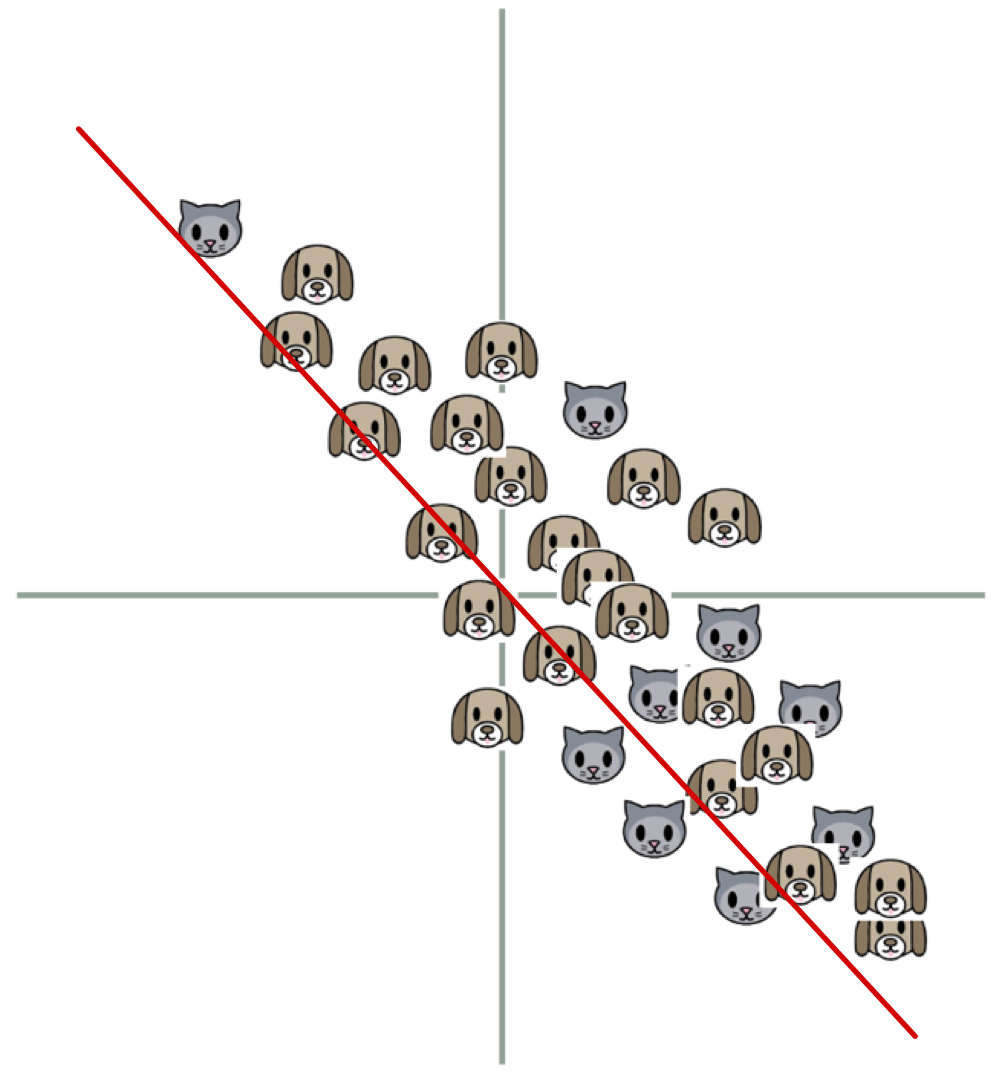
\includegraphics[width=0.6\textwidth]{image_06}
            \end{figure}

        \subsection{Problem 4.2. (2 Points)}
            If the data has 1,000 dimensions, and 100 samples, how many PCA projections can there be?

            \vspace{1em}

            \noindent \underline{\textbf{Ans.}} There can be 99 PCA projections because
            it can be determined by $\min(N - 1, D)$ where $N$ is a number of samples and $D$ is a number of data dimensions.

        \subsection{Problem 4.3. (2 Points)}
            If I increase the amount of samples to 10,000, how many PCA projections can there be?

            \vspace{1em}

            \noindent \underline{\textbf{Ans.}} There can be 1,000 PCA projections because
            it can be determined by $\min(N - 1, D)$ where $N$ is a number of samples and $D$ is a number of data dimensions.

    \pagebreak

        \subsection{Problem 4.4. (2 Points)}
            What is the size of the covariance matrix if the data has 1,000 dimensions?

            \vspace{1em}

            \noindent \underline{\textbf{Solution}}

            \vspace{0.25em}

            The dataset $\mathbf{X}$ has $N$ samples and $D$ dimensions (features) and can be written as a $N \times D$ matrix below.
            \begin{align*}
                \mathbf{X} =
                \begin{bmatrix}
                    X_{11} & X_{12} & \dots & X_{1D} \\
                    X_{21} & X_{22} & \dots & X_{2D} \\
                    \vdots & \vdots & \ddots & \vdots \\
                    X_{N1} & X_{N2} & \dots & X_{ND} \\
                \end{bmatrix}
            \end{align*}

            From the definition of covariance on two specific feature (column $i$ and $j$) is the following equation.
            \begin{align*}
                \text{Cov}(i, j) &= \frac{1}{N - 1} \sum_{k = 1}^{N}(X_{ki} - \mu_{i})(X_{kj} - \mu_{j}) \\[1em]
                \intertext{The mean ($\mu_{i}, \mu_{j}$) are equal to 0 because the data are centered at the origin point}
                \text{Cov}(i, j) &= \frac{1}{N - 1} \sum_{k = 1}^{N} X_{ki} X_{kj} \\[1em]
                \text{Cov}(i, j) &= \frac{1}{N - 1}
                    \begin{bmatrix}
                        X_{1i} \\
                        X_{2i} \\
                        \vdots \\
                        X_{Ni} \\
                    \end{bmatrix}^{T}
                    \cdot
                    \begin{bmatrix}
                        X_{1j} \\
                        X_{2j} \\
                        \vdots \\
                        X_{Nj} \\
                    \end{bmatrix}
            \end{align*}

            From the equation above, it is the definition of dot product of feature $i$ and $j$ which means the covariance matrix can be written as
            $$\Sigma = \frac{1}{N - 1} {\mathbf{X}}^{T} \mathbf{X}$$

            Since the dataset matrix $\mathbf{X}$ has $N \times D$ size, $\mathbf{X}^{T}$ has $D \times N$ size.
            Therefore, ${\mathbf{X}}^{T} \mathbf{X}$ has $D \times D$ size which in this problem has $D$ equals to 1000.

            \vspace{0.5em}

            \noindent \underline{\textbf{Ans.}} The size of covariance matrix is $1000 \times 1000$.

    \pagebreak

        \subsection{Problem 4.5. (2 Points)}
            From the problem 4.3., what is the size of the Gram matrix?
            If we want to compute the PCA, should we compute from the Gram or from the covariance matrix?

            \vspace{1em}

            \noindent \underline{\textbf{Solution}}

            \vspace{0.25em}

            The dataset $\mathbf{X}$ has $N$ samples and $D$ dimensions (features) and can be written as a $N \times D$ matrix below.
            \begin{align*}
                \mathbf{X} =
                \begin{bmatrix}
                    X_{11} & X_{12} & \dots & X_{1D} \\
                    X_{21} & X_{22} & \dots & X_{2D} \\
                    \vdots & \vdots & \ddots & \vdots \\
                    X_{N1} & X_{N2} & \dots & X_{ND} \\
                \end{bmatrix}
            \end{align*}

            \noindent According to the Singular Value Decomposition (SVD) of a $N \times D$ size matrix $\mathbf{X}$
            \begin{itemize}
                \item $U$ is an $N \times N$ orthogonal matrix which its left singular vector (columns) are perpendicular.
                \item $\Sigma$ is a $N \times D$ diagonal matrix containing the singular values ($\sigma$)
                \item $V$ is a $D \times D$ orthogonal matrix which its right singular vector (columns) are perpendicular.
            \end{itemize}
            \begin{align*}
                \intertext{Express $U$ in terms of $\mathbf{X}$, $\Sigma$ and $V$}
                \mathbf{X} &= U \Sigma V^T
                \intertext{Multiple both size with matrix $V$}
                \mathbf{X} V &= U \Sigma V^T V \\
                \intertext{Because $V$ is an orthogonal matrix, $V^T V = V V^T = I$}
                \mathbf{X} V &= U \Sigma \\
                U &= \mathbf{X} V {\Sigma}^{-1} \tag{1} \\[1em]
                \intertext{Express $V$ in terms of $\mathbf{X}$, $\Sigma$ and $U$}
                \mathbf{X} &= U \Sigma V^T \\
                \intertext{Multiple both size with matrix $U^T$}
                U^T \mathbf{X} &= U^T U \Sigma V^T \\
                \intertext{Because $U$ is an orthogonal matrix, $U^T U = U U^T = I$}
                U^T \mathbf{X} &= \Sigma V^T \\
                V^T &= \Sigma^{-1} U^T \mathbf{X} \\
                \intertext{Apply the transpose rule: $(AB)^T = B^T A^T$ and $(A^T)^T = A$}
                V &= (\Sigma^{-1} U^T \mathbf{X})^T \\
                \intertext{$\Sigma$ is a diagonal matrix which means $\Sigma^T = \Sigma$}
                V &= \mathbf{X}^T U \Sigma^{-1} \tag{2}
            \end{align*}

    \pagebreak

            \noindent This is a definition of a eigendecomposition of a $n \times n$ matrix $A$
            $$A = Q \Lambda Q^{-1}$$
            \begin{itemize}
                \item $Q$ is an $n \times n$ matrix containing eigenvectors.
                \item $\Lambda$ is a $n \times n$ diagonal matrix containing the corresponding eigenvalues.
            \end{itemize}

            \vspace{1em}

            \noindent Consider the eigendecomposition of covariance matrix ($\mathbf{X}^T \mathbf{X}$)
            \begin{align*}
                \mathbf{X}^T \mathbf{X} &= (U \Sigma V^T)^T (U \Sigma V^T) \\
                \intertext{Apply the transpose rule: $(AB)^T = B^T A^T$ and $(A^T)^T = A$}
                \mathbf{X}^T \mathbf{X} &= V \Sigma^T U^T U \Sigma V^T \\
                \intertext{$\Sigma$ is a diagonal matrix which means $\Sigma^T = \Sigma$}
                \mathbf{X}^T \mathbf{X} &= V \Sigma U^T U \Sigma V^T \\
                \intertext{$U$ is an orthogonal matrix which means $U^T U = U U^T = I$}
                \mathbf{X}^T \mathbf{X} &= V \Sigma I \Sigma V^T \\
                \mathbf{X}^T \mathbf{X} &= V \Sigma^2 V^T \tag{3}
            \end{align*}
            \begin{itemize}
                \item $V$ is a matrix containing eigenvectors.
                \item $\Sigma^2$ is a diagonal matrix containing the corresponding eigenvalues.
                \item Note that $V$ is an orthogonal matrix which $V^T = V^{-1}$
            \end{itemize}

            \vspace{1em}

            Gram matrix is defined as a matrix of all possible dot product of a set of vectors which are samples (rows) in this problem
            and can be written as
            $$\mathbf{G} = \mathbf{X} \mathbf{X}^T$$

            \noindent Consider the eigendecomposition of Gram matrix ($\mathbf{X} \mathbf{X}^T$)
            \begin{align*}
                \mathbf{X} \mathbf{X}^T &= (U \Sigma V^T) (U \Sigma V^T)^T \\
                \intertext{Apply the transpose rule: $(AB)^T = B^T A^T$ and $(A^T)^T = A$}
                \mathbf{X} \mathbf{X}^T &= U \Sigma V^T V \Sigma^T U^T \\
                \intertext{$\Sigma$ is a diagonal matrix which means $\Sigma^T = \Sigma$}
                \mathbf{X} \mathbf{X}^T &= U \Sigma V^T V \Sigma U^T \\
                \intertext{$U$ is an orthogonal matrix which means $U^T U = U U^T = I$}
                \mathbf{X} \mathbf{X}^T &= U \Sigma I \Sigma U^T \\
                \mathbf{X} \mathbf{X}^T &= U \Sigma^2 U^T \tag{4}
            \end{align*}
            \begin{itemize}
                \item $U$ is a matrix containing eigenvectors.
                \item $\Sigma^2$ is a diagonal matrix containing the corresponding eigenvalues.
                \item Note that $U$ is an orthogonal matrix which $U^T = U^{-1}$
            \end{itemize}

    \pagebreak

        \noindent According to those equations
        \begin{align*}
            U &= \mathbf{X} V {\Sigma}^{-1} \tag{1} \\
            V &= \mathbf{X}^T U \Sigma^{-1} \tag{2} \\
            \mathbf{X}^T \mathbf{X} &= V \Sigma^2 V^T \tag{3} \\
            \mathbf{X} \mathbf{X}^T &= U \Sigma^2 U^T \tag{4}
        \end{align*}

        \noindent To compute the PCA using the Gram matrix $\mathbf{X} \mathbf{X}^T$, it has to follow these steps
        \begin{enumerate}
            \item Perform an eigendecomposition to the gram matrix $\mathbf{X} \mathbf{X}^T$ by using the equation (4)
            and get its eigenvector matrix $U$ and corresponding eigenvalues matrix $\Sigma^2$.
            \item Calculate the matrix $V$ by the equation (2).
            \item Use $U$, $V$ and $\Sigma$ from the previous steps to compute PCA.
        \end{enumerate}

        \vspace{1em}

        \noindent To compute the PCA using the covariance matrix $\mathbf{X}^T \mathbf{X}$, it has to follow these steps
        \begin{enumerate}
            \item Perform an eigendecomposition to the covariance matrix $\mathbf{X}^T \mathbf{X}$ by using the equation (3)
            and get its eigenvector matrix $V$ and corresponding eigenvalues matrix $\Sigma^2$.
            \item Calculate the matrix $U$ by the equation (1).
            \item Use $U$, $V$ and $\Sigma$ from the previous steps to compute PCA.
        \end{enumerate}

        \vspace{1em}

        Those two methods has similar process to compute the PCA which are performing an eigendecomposition then finding another singular matrix.
        However, it is significantly different in both computation and memory usage aspects.
        \begin{itemize}
            \item \textbf{Covariance Matrix} is calculated by $\mathbf{X}^T \mathbf{X}$ which has $1000 \times 1000$ size.
            \item \textbf{Covariance Matrix} takes ${1000}^3$ or ${10}^9$ operations to perform a eigendecomposition.
            \item \textbf{Gram Matrix} is calculated by $\mathbf{X} \mathbf{X}^T$ which has $10000 \times 10000$ size.
            \item \textbf{Gram Matrix} takes ${10000}^3$ or ${10}^{12}$ operations to perform a eigendecomposition.
        \end{itemize}
        \noindent Therefore, having PCA computed by the covariance matrix is theoretically 1,000 times faster than by the Gram matrix.

        \vspace{1em}

        \noindent \underline{\textbf{Ans.}} The size of Gram matrix is $10000 \times 10000$
        and having PCA computed by the covariance matrix is a better choice.

    \pagebreak

    \section{Problem 5 (18 Points)}
        Consider the following neural network code.

        \subsection{Problem 5.1. (5 Points)}
            Draw a picture of the \texttt{FeedForwardNN} network. Be sure to specify the dimensions of the input/output of each layer.
            \begin{codeblock}{}
                class FeedForwardNN(nn.Module):
                    def __init__(self, hidden_size=200):
                        super(FeedForwardNN, self).__init__()
                        self.ff1 = nn.Linear(30, 80)
                        self.ff2 = nn.Linear(80, 90)
                        self.ff3 = nn.Linear(90, 90)
                        self.out = nn.Linear(90, 1)

                    def forward(self, x):
                        hd1 = F.relu(self.ff1(x))
                        hd2 = F.relu(self.ff2(hd1))
                        y = F.relu(self.ff3(hd2))
                        y = self.out(y)
                        return y
            \end{codeblock}

            \noindent The answer is in the next page $\rightarrow$

    \pagebreak

            \noindent \underline{\textbf{Answer}}
            \begin{figure}[h]
                \centering
                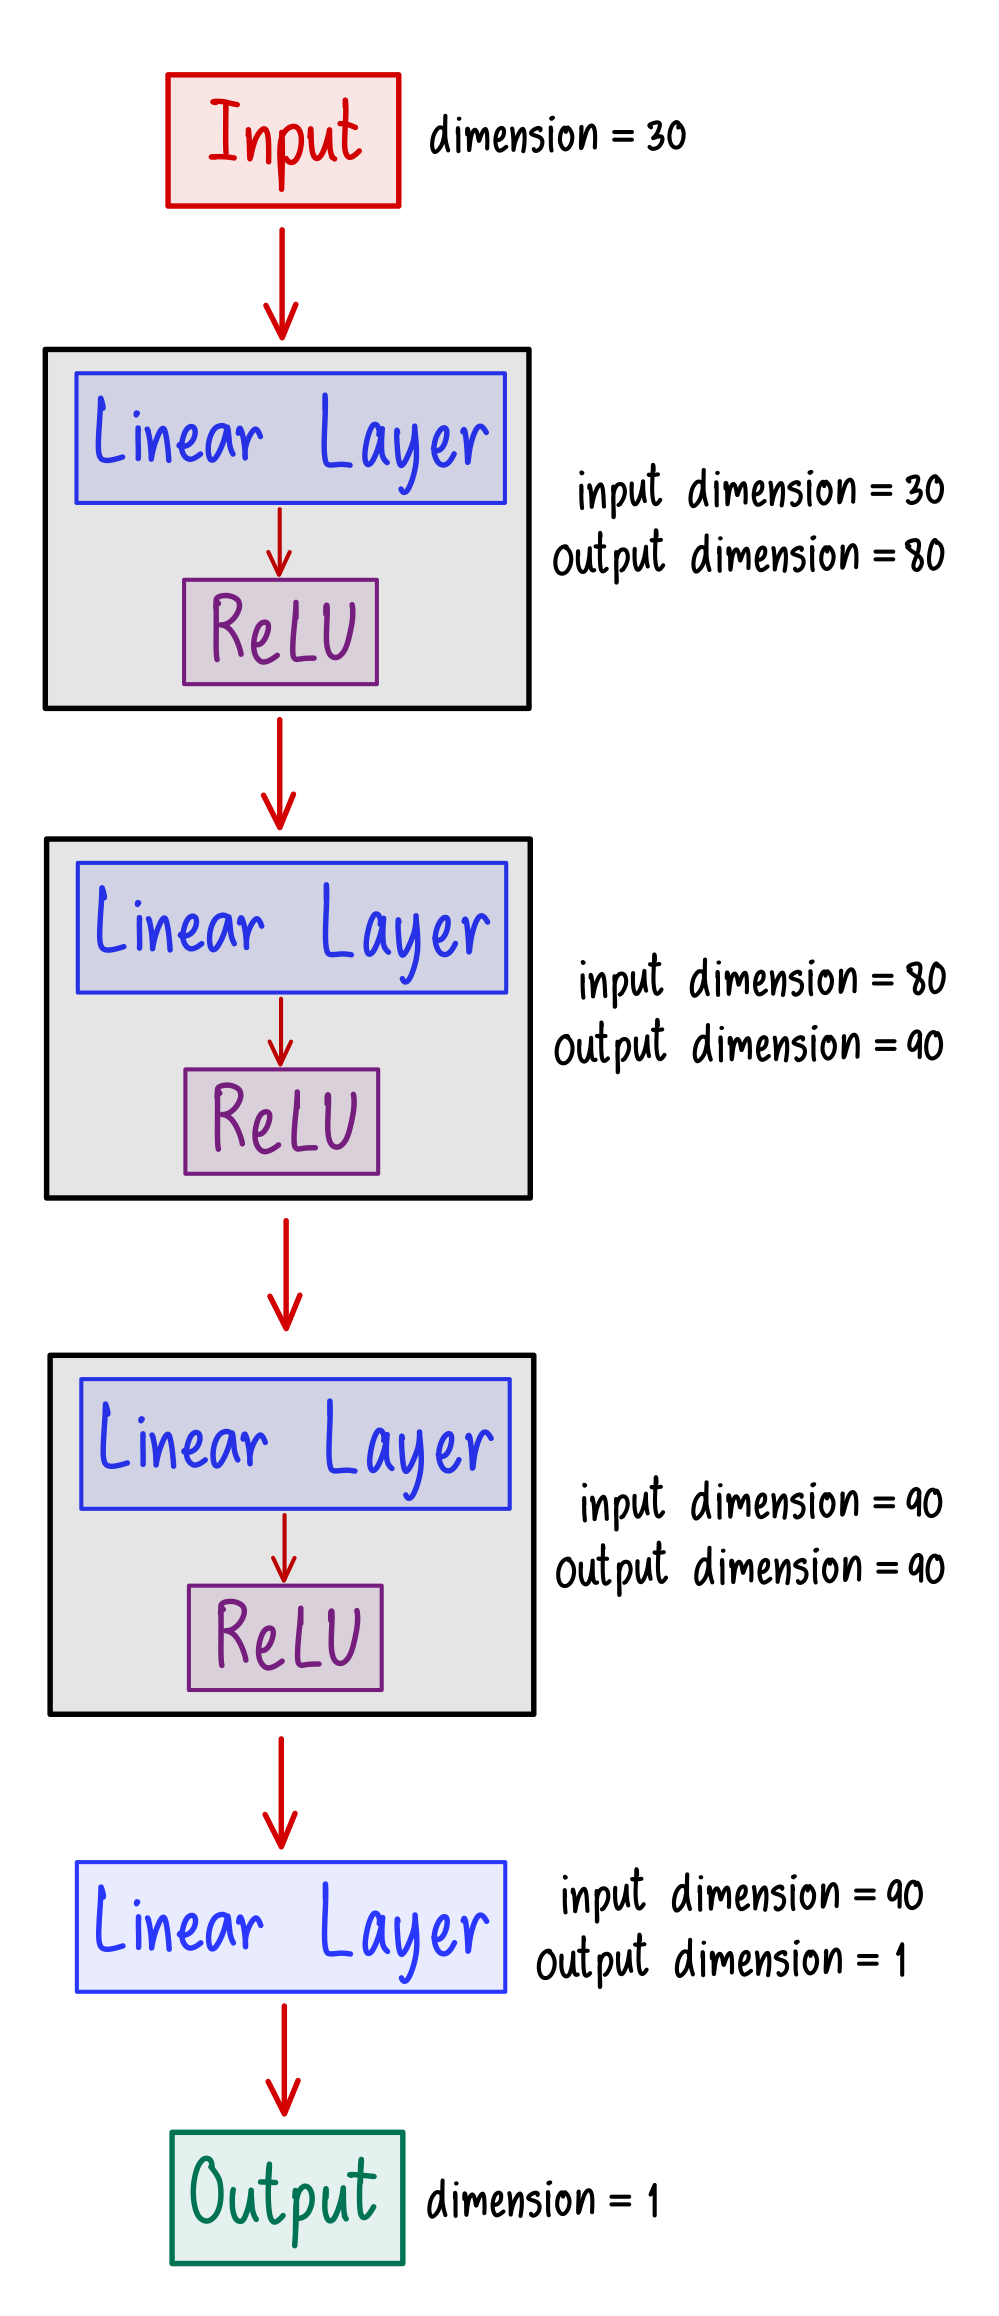
\includegraphics[width=0.5\textwidth]{image_07}
            \end{figure}

    \pagebreak

        \subsection{Problem 5.2. (3 Points)}
            How many parameters does the layer \texttt{ff2} have?

            \vspace{1em}

            \noindent \underline{\textbf{Solution}}

            \vspace{0.25em}

            The PyTorch linear layer computes a matrix multiplication and adds a bias by default: $y = x A^T + b$.
            In \texttt{ff2} layer has 80 input nodes and 90 output nodes, so the parameters can be calculated as follows.
            \begin{table}[h]
                \centering
                \begin{tabular}{|c|c|}
                    \hline
                    Category & Parameters \\
                    \hline \hline
                    Weights & $80 \times 90 = 7200$ \\
                    \hline
                    Bias & $1 \times 90 = 90$ \\
                    \hline
                \end{tabular}
            \end{table}

            \noindent \underline{\textbf{Ans.}} The \texttt{ff2} layer has 7290 parameters.

        \subsection{Problem 5.3. (2 Points)}
            If the mini-batch is of size 64, what should be the size of the input tensor?

            \vspace{1em}

            \noindent \underline{\textbf{Ans.}} The \texttt{ff2} Since the batch size is 64 and the first layer (\texttt{ff1}) has 30 input nodes,
            the size of the input tensor is (64, 30).

        \subsection{Problem 5.4. (5 Points)}
            Draw a picture of the \texttt{FeedForwardNN2} network. What should A and B be?
            \begin{codeblock}{}
                class FeedForwardNN2(nn.Module):
                    def __init__(self, hidden_size=200):
                        super(FeedForwardNN2, self).__init__()
                        self.ff1 = nn.Linear(30, 80)
                        self.ff2 = nn.Linear(A, 80)
                        self.ff3 = nn.Linear(B, 90)
                        self.out = nn.Linear(90, 1)

                    def forward(self, x):
                        hd1 = self.ff1(x)
                        hd2 = self.ff2(x)
                        hd3 = F.relu(hd1+hd2)
                        y = F.relu(self.ff3(hd3))
                        y = self.out(y)
                        return y
            \end{codeblock}

        \noindent The answer is in the next page $\rightarrow$

    \pagebreak

            \noindent \underline{\textbf{Answer}}

            \vspace{0.25em}

            The $A$ should be 30 because it needs to match with the input (\texttt{x}) dimensions
            and $B$ should be 80 because it needs to match with the \texttt{ff1} and \texttt{ff2} output dimensions.
            \begin{figure}[h]
                \centering
                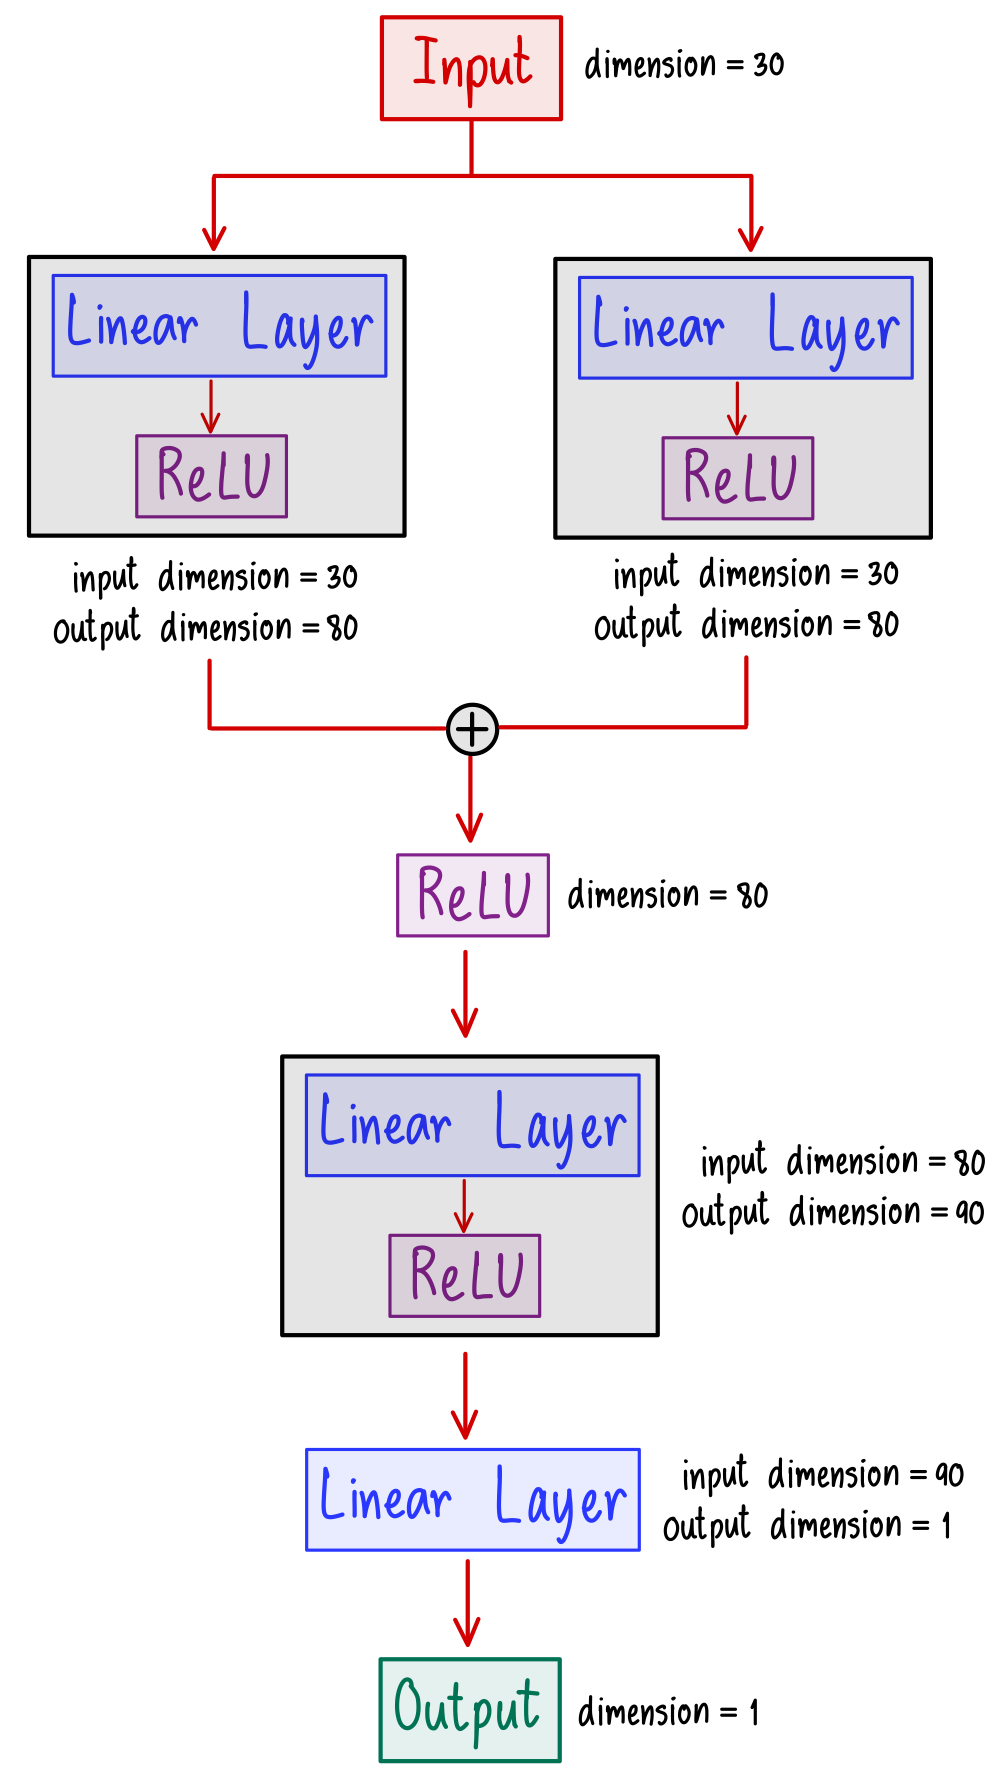
\includegraphics[width=0.6\textwidth]{image_08}
            \end{figure}

    \pagebreak
        \subsection{Problem 5.5. (3 Points)}
            In \texttt{FeedForwardNN2}, the output from \texttt{ff1} and \texttt{ff2} are then summed together to make an output of size 80.
            How is this different from having just one single linear layer with 80 outputs (instead of 2)?
            Are they ultimately the same?

            \vspace{1em}

            \noindent \underline{\textbf{Solution}}

            \vspace{0.25em}

            The model has two linear layers, \texttt{ff1} and \texttt{ff2} and then sums it, which can be written as the equation below.
            (Given that the weights are $W_1$, $W2$ and the bias are $b_1$, $b_2$)
            \begin{align*}
                (W_1 x^T + b_1) + (W_2 x^T + b_2) &= (W_1 + W_2)x^T + (b_1 + b_2) \\
                (W_1 x^T + b_1) + (W_2 x^T + b_2) &= W_{\text{total}} x^T + b_{\text{total}}
            \end{align*}
            This equation shows that the sum of \texttt{ff1} and \texttt{ff2} layers which have the same functionality
            is equivalent with a single linear layer.
            \begin{align*}
                \intertext{Calculate the gradient of loss with respect to $W_1$}
                \frac{\partial L}{\partial W_1} &= \frac{\partial L}{\partial y} \cdot \frac{\partial y}{\partial W_1} \\[1em]
                \frac{\partial L}{\partial W_1} &= \frac{\partial L}{\partial y} \cdot \frac{\partial}{\partial W_1} (W_1 x^T + W_2 x^T + (b_1 + b_2)) \\[1em]
                \frac{\partial L}{\partial W_1} &= \frac{\partial L}{\partial y} \cdot x^T \tag{1} \\[1em]
                \intertext{Calculate the gradient of loss with respect to $W_2$}
                \frac{\partial L}{\partial W_2} &= \frac{\partial L}{\partial y} \cdot \frac{\partial y}{\partial W_2} \\[1em]
                \frac{\partial L}{\partial W_2} &= \frac{\partial L}{\partial y} \cdot \frac{\partial}{\partial W_2} (W_1 x^T + W_2 x^T + (b_1 + b_2)) \\[1em]
                \frac{\partial L}{\partial W_2} &= \frac{\partial L}{\partial y} \cdot x^T \tag{2}
            \end{align*}

            Considering the backpropagation process, the gradient of both are identical which means the weights of both layers are always updated by the exact same amount.
            Therefore, it is clearly shows that this is the same as the single layer but wastes more computational and memory usage.

            \vspace{1em}

            \noindent \underline{\textbf{Ans.}} Creating 2 identical linear layers and sum afterwards is not different from creating a single linear layer.
            Moreover, it wastes more computational and memory usage.

    \pagebreak

    \section{Problem 6 (12 Points)}
        \subsection{Problem 6.1. (2 Points)}
            Given an input of size $10 \times 10 \times 3$ ($H \times W \times C$).
            If we apply a 2D CNN of size $3 \times 3$, stride 2, padding 1 with 5 filters, specify the size of the output tensor.

            \vspace{1em}

            \noindent \underline{\textbf{Solution}}

            \vspace{0.25em}

            \noindent To find the size of the output tensor after a 2D convolution, use this following formula
            $$O = \left\lfloor \frac{I - K + 2P}{S} \right\rfloor + 1$$
            \begin{itemize}
                \item $O$ is the output size
                \item $I$ is the input size
                \item $K$ is the kernel size
                \item $F$ is the padding
                \item $S$ is the stride
            \end{itemize}
            $$O = \left\lfloor \frac{10 - 3 + 2(1)}{2} \right\rfloor + 1 = 5$$

            \noindent The depth (channels) of the output is always equal to the number of filters applied.

            \vspace{1em}

            \noindent \underline{\textbf{Ans.}} The size of the output tensor is $5 \times 5 \times 5$

    \pagebreak

        \subsection{Problem 6.2. (2 Points)}
            Given a convolution neural network with connections
            \begin{enumerate}
                \item \texttt{Input}
                \item \texttt{conv2d} $3 \times 3$ with stride 1
                \item \texttt{maxpool} $2 \times 2$
                \item \texttt{conv2d} $2 \times 2$ with stride 1
            \end{enumerate}
            Find the receptive field of the final convolution layer

            \vspace{1em}

            \noindent \underline{\textbf{Solution}}

            \vspace{0.25em}

            The receptive field in Convolutional Neural Network (CNN) is the specific region of the input image,
            measured in pixels, that a particular feature (neuron) sees and is affected by.
            The image below shows that a $1 \times 1$ pixel in layer 3 sees the $5 \times 5$ pixels of the original input.
            \begin{figure}[h]
                \centering
                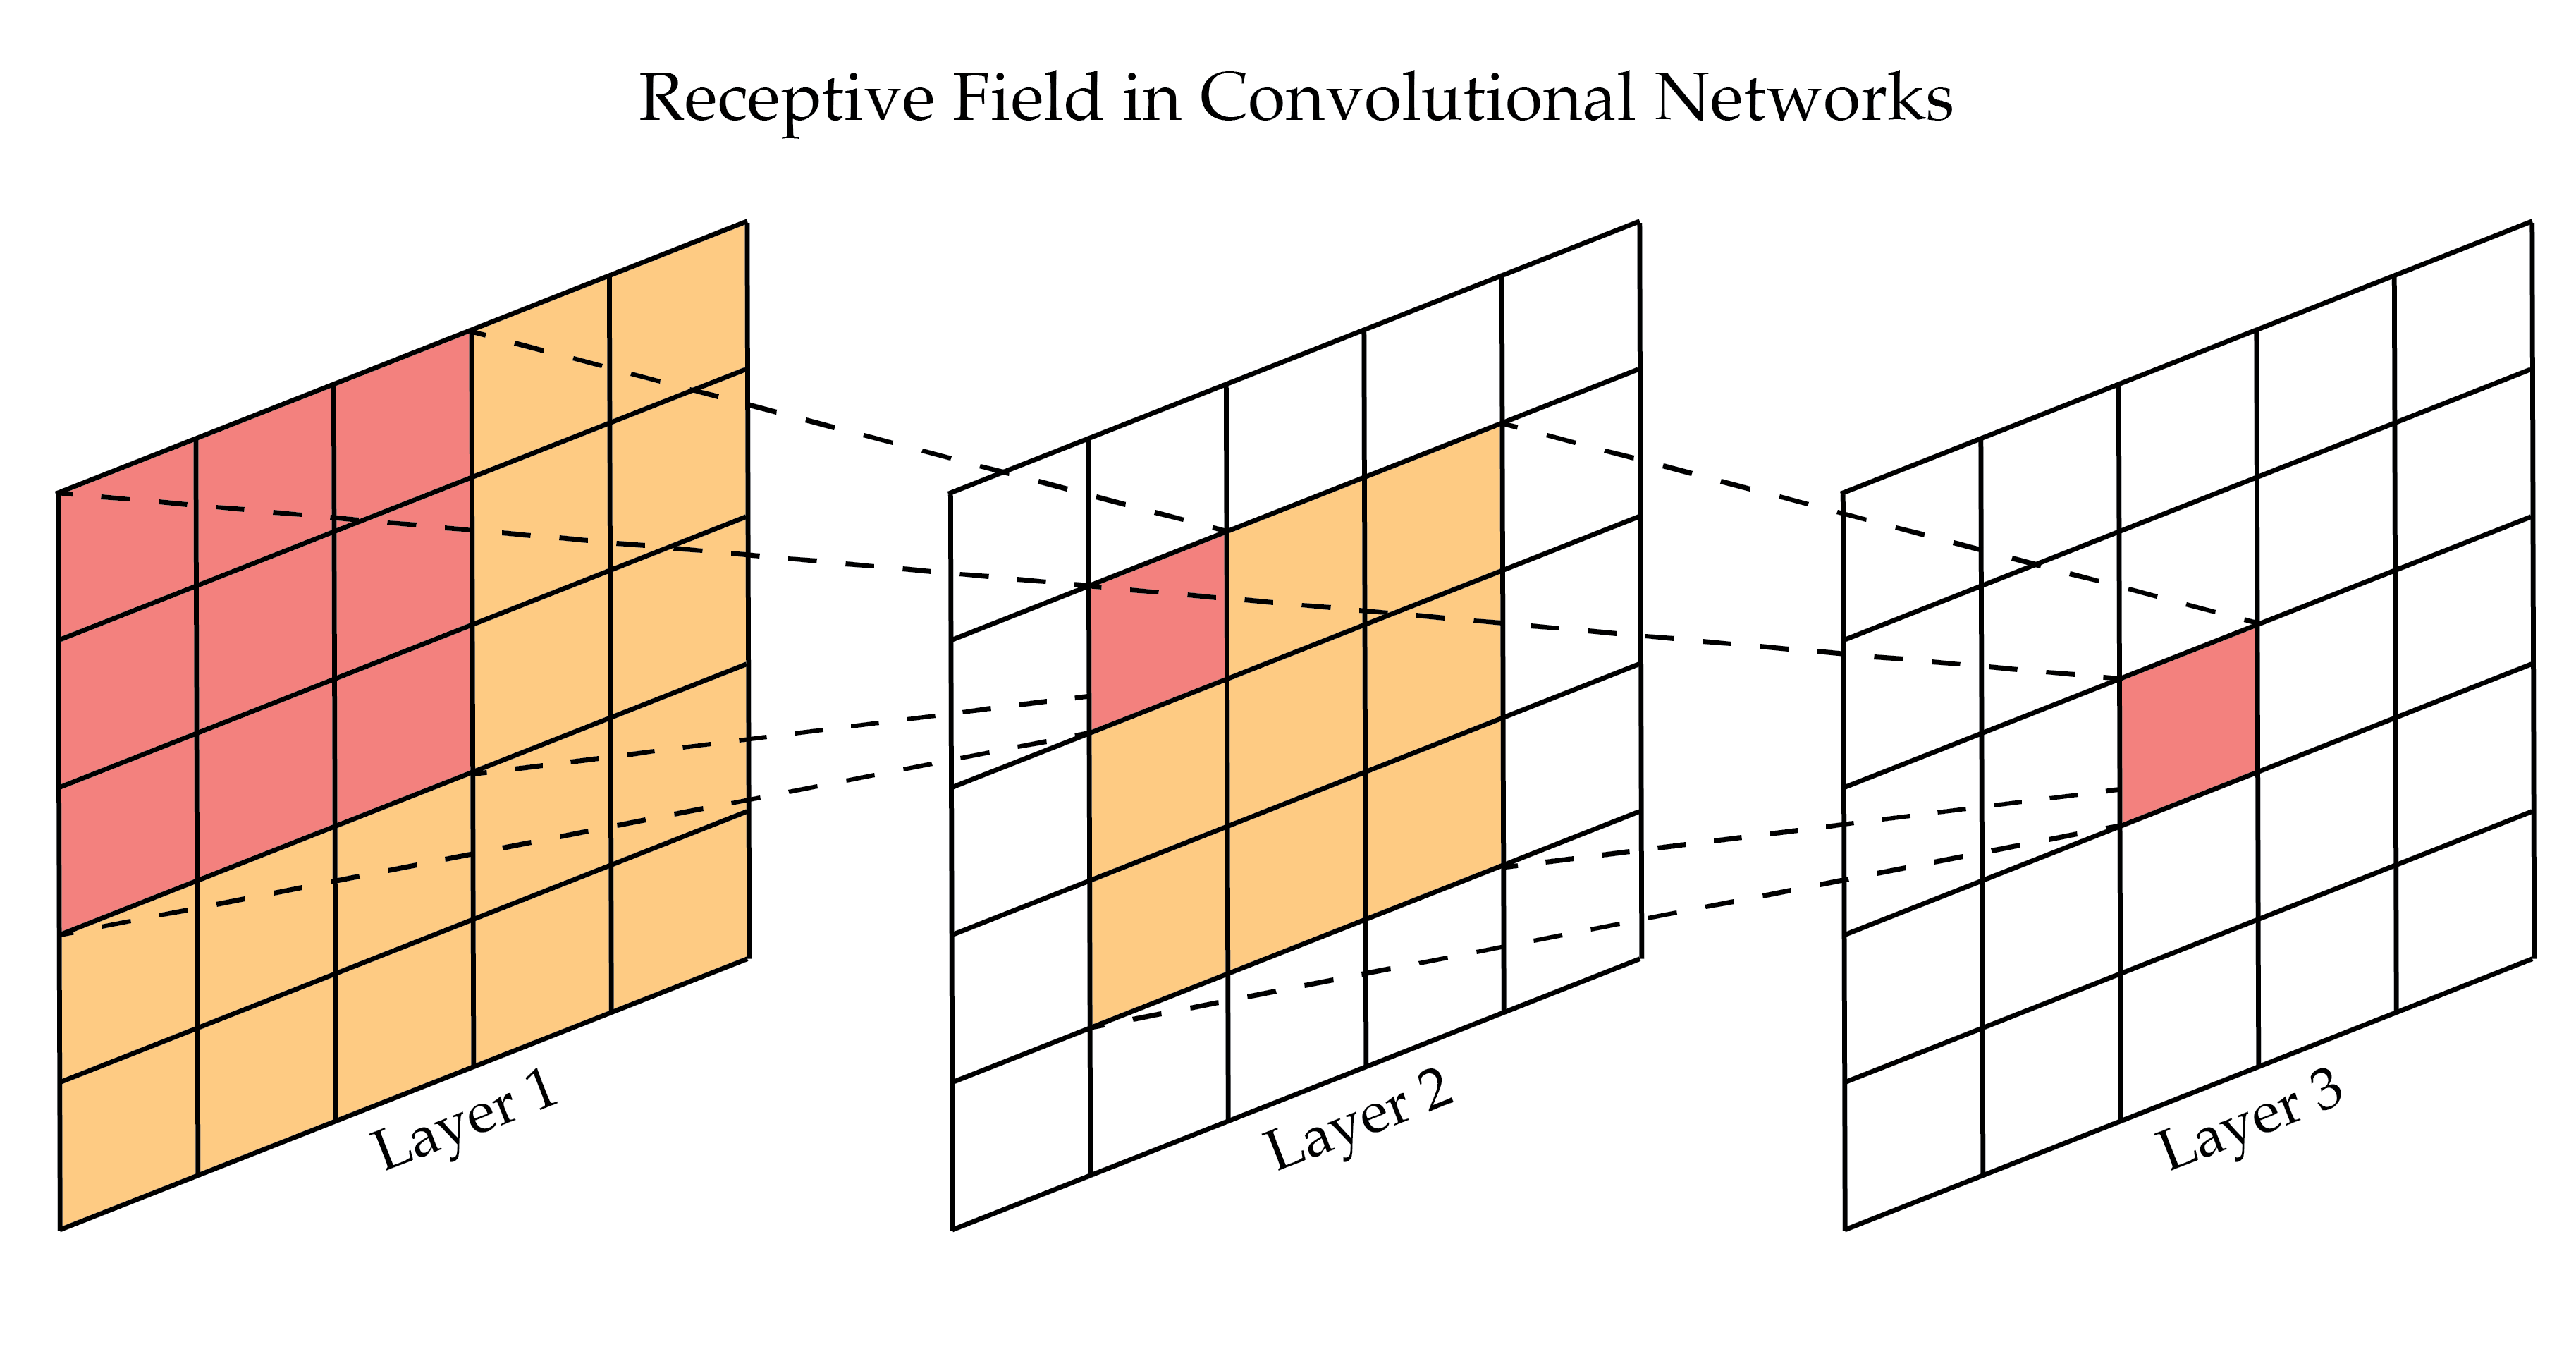
\includegraphics[width=0.6\textwidth]{image_09}
            \end{figure}

            The formula to calculate the reception field is
            $$r_l = r_{l - 1} + (k_l - 1) \times j_{l - 1}$$
            $$j_l = j_{l - 1} \times s_l$$
            \begin{itemize}
                \item $r_l$ is the reception field of the layer $l$
                \item $j_l$ is the jump (accumulated stride) of the layer $l$
                \item $s_l$ is the stride of the layer $l$
            \end{itemize}

            \begin{enumerate}
                \item \textbf{Input Layer} starts with $r_0 = 1$ and $j_0 = 1$.
                \item \textbf{Convolutional Layer} with $3 \times 3$ kernel size and stride equals to 1
                \begin{itemize}
                    \item $k_1 = 3$ and $s_1 = 1$
                    \item $j_1 = j_0 \times s_1 = 1$
                    \item $r_1 = r_0 + (k_1 - 1) \times j_0$ \\
                    $r_1 = 1 + (3 - 1) \times 1 = 3$
                \end{itemize}

    \pagebreak

                \item \textbf{Max Pooling Layer} with $2 \times 2$ kernel size and stride equals to 2
                \begin{itemize}
                    \item $k_2 = 2$ and $s_2 = 2$
                    \item $j_2 = j_1 \times s_2$ \\
                    $j_2 = 1 \times 2 = 2$
                    \item $r_2 = r_1 + (k_2 - 1) \times j_1$ \\
                    $r_2 = 3 + (2 - 1) \times 1 = 4$
                \end{itemize}
                \item \textbf{Convolutional Layer} with $2 \times 2$ kernel size and stride equals to 1
                \begin{itemize}
                    \item $k_3 = 2$ and $s_3 = 1$
                    \item $j_3 = j_2 \times s_3$ \\
                    $j_3 = 2 \times 1 = 2$
                    \item $r_3 = r_2 + (k_3 - 1) \times j_2$ \\
                    $r_3 = 4 + (2 - 1) \times 2 = 6$
                \end{itemize}
            \end{enumerate}

            \noindent Since $r_3 = 6$, the final reception field has $6 \times 6$ size.

            \vspace{1em}

            \noindent \underline{\textbf{Ans.}} The size of the final reception field is $6 \times 6$

    \pagebreak

        \subsection{Problem 6.3. (4 Points)}
            If we apply the following kernel to the input, what is the output? Assume the bias is 0, use a stride = 2, and no padding.
            \begin{table}[h]
                \centering
                \begin{tabular}{|c|c|c|c|c|}
                    \hline
                    1 & 2 & 3 & 0 & 1 \\
                    \hline
                    4 & 1 & 0 & 2 & 3 \\
                    \hline
                    1 & 3 & 2 & 1 & 0 \\
                    \hline
                    0 & 1 & 4 & 2 & 1 \\
                    \hline
                    2 & 3 & 1 & 0 & 4 \\
                    \hline
                \end{tabular}
                \caption{Input}
            \end{table}

            \begin{table}[h]
                \centering
                \begin{tabular}{|c|c|c|}
                    \hline
                    1 & 0 & -1 \\
                    \hline
                    0 & 1 & 0 \\
                    \hline
                    -1 & 0 & 1 \\
                    \hline
                \end{tabular}
                \caption{Kernel}
            \end{table}

                \subsubsection{The first convolution}
                    First, apply the kernel (filter) just on the top left of the input
                    \begin{align*}
                        {X}_{11} &=
                        \begin{bmatrix}
                            1 & 2 & 3 \\
                            4 & 1 & 0 \\
                            1 & 3 & 2 \\
                        \end{bmatrix}
                        \ast
                        \begin{bmatrix}
                            1  & 0 & -1 \\
                            0  & 1 & 0  \\
                            -1 & 0 & 1  \\
                        \end{bmatrix}
                        \\[1em]
                        {X}_{11} &= [1(1) + 2(0) + 3(-1)] + [4(0) + 1(1) + 0(0)] + [1(-1) + 3(0) + 2(1)] \\
                        {X}_{11} &= 0
                    \end{align*}

                \subsubsection{The second convolution}
                    Then, shift the kernel (filter) right by 2 steps from the top left on the input.
                    \begin{align*}
                        {X}_{12} &=
                        \begin{bmatrix}
                            3 & 0 & 1 \\
                            0 & 2 & 3 \\
                            2 & 1 & 0 \\
                        \end{bmatrix}
                        \ast
                        \begin{bmatrix}
                            1  & 0 & -1 \\
                            0  & 1 & 0  \\
                            -1 & 0 & 1  \\
                        \end{bmatrix}
                        \\[1em]
                        {X}_{12} &= [3(1) + 0(0) + 1(-1)] + [0(0) + 2(1) + 3(0)] + [2(-1) + 1(0) + 0(1)] \\
                        {X}_{12} &= 2
                    \end{align*}

                \subsubsection{The third convolution}
                    Then, shift the kernel (filter) down by 2 steps from the top left on the input.
                    \begin{align*}
                        {X}_{21} &=
                        \begin{bmatrix}
                            1 & 3 & 2 \\
                            0 & 1 & 4 \\
                            2 & 3 & 1 \\
                        \end{bmatrix}
                        \ast
                        \begin{bmatrix}
                            1  & 0 & -1 \\
                            0  & 1 & 0  \\
                            -1 & 0 & 1  \\
                        \end{bmatrix}
                        \\[1em]
                        {X}_{21} &= [1(1) + 3(0) + 2(-1)] + [0(0) + 1(1) + 4(0)] + [2(-1) + 3(0) + 1(1)] \\
                        {X}_{21} &= -1
                    \end{align*}

                \subsubsection{The forth convolution}
                    Finally, shift the kernel (filter) down by 2 steps and shift right by 2 steps from the top left on the input.
                    \begin{align*}
                        {X}_{22} &=
                        \begin{bmatrix}
                            2 & 1 & 0 \\
                            4 & 2 & 1 \\
                            1 & 0 & 4 \\
                        \end{bmatrix}
                        \ast
                        \begin{bmatrix}
                            1  & 0 & -1 \\
                            0  & 1 & 0  \\
                            -1 & 0 & 1  \\
                        \end{bmatrix}
                        \\[1em]
                        {X}_{22} &= [2(1) + 1(0) + 0(-1)] + [4(0) + 2(1) + 1(0)] + [1(-1) + 0(0) + 4(1)] \\
                        {X}_{22} &= 7
                    \end{align*}

                \subsubsection{Result}
                    After the convolution, we got this as a final output matrix.
                    $$
                        \begin{bmatrix}
                            0 & 2 \\
                            -1 & 7 \\
                        \end{bmatrix}
                    $$

        \subsection{Problem 6.4. (5 Points)}
            You want to train a simple three-layer (two hidden layers) neural network for a 10-class classification.
            Each hidden layer has 100 neurons. The input size is 80. How many parameters are in this neural network?

            \vspace{1em}

            \noindent \underline{\textbf{Solution}}

            \vspace{0.25em}

            \begin{table}[h]
                \centering
                \begin{tabular}{|c|c|c|c|c|c|}
                    \hline
                    \textbf{Layers} & \textbf{Input} & \textbf{Output} & \textbf{Weights} & \textbf{Bias} & \textbf{Total} \\
                    \hline \hline
                    Hidden Layer 1 & 80 & 100 & $80 \times 100 = 8,000$ & 100 & 8,100 \\
                    \hline
                    Hidden Layer 2 & 100 & 100 & $100 \times 100 = 10,000$ & 100 & 10,100 \\
                    \hline
                    Output Layer & 100 & 10 & $100 \times 10 = 1,000$ & 10 & 1,010 \\
                    \hline
                \end{tabular}
            \end{table}
            \noindent Total parameters = 8,100 + 10,100 + 1,010 = 19,210

			\vspace{1em}

            \noindent \underline{\textbf{Ans.}} This neural network has 19,210 parameters.

	\pagebreak

        \subsection{Problem 6.5. (2 Points)}
            From the problem 6.4, what are the possible hyper-parameters that you can change?
            List at least 4 of them.

            \vspace{1em}

            \noindent \underline{\textbf{Answer}}

            \begin{enumerate}
                \item \textbf{Learning Rate}: step size at each iteration to move for the minimum loss.
                \item \textbf{Neurons in Layer}: increase or decrease neural network capacity.
                \item \textbf{Batch Size}: number of training samples used in one iteration.
                \item \textbf{Epochs}: number of times that neural network leans through the entire training dataset.
                \item \textbf{Activation Function}: the non-linearity function used in the hidden layer (e.g. ReLU, Sigmoid).
            \end{enumerate}

\end{document}